\chapter{Configurazione Sperimentale e Risultati}

Il presente capitolo descrive la configurazione adottata per la generazione del dataset sintetico, i comandi utilizzati per produrre le immagini nelle diverse modalità, e i risultati ottenuti in termini di tempi di generazione e varietà del dataset prodotto.

\section{Ambiente di Esecuzione}

\subsection{Hardware e Software}

I benchmark riportati in questo capitolo sono stati eseguiti sulla seguente configurazione hardware:

\begin{itemize}
    \item \textbf{CPU:} \texttt{[Amd Ryzen 5700X, 8 core]}
    \item \textbf{RAM:} \texttt{[16 GB DDR4]}
    \item \textbf{Sistema Operativo:} \texttt{[Windows 10]}
    \item \textbf{Python:} 3.12.10
    \item \textbf{TensorFlow:} 2.x (modalità compatibilità TF1, esecuzione CPU-only)
\end{itemize}

\subsection{Dataset di Input: PTB-XL}

Il dataset utilizzato come sorgente dei segnali ECG è \textbf{PTB-XL}~\cite{PhysioNet-ptb-xl-1.0.3}, una raccolta pubblica disponibile su PhysioNet contenente 21\,799 registrazioni ECG a 12 derivazioni della durata di 10 secondi ciascuna, acquisite su 18\,869 pazienti. Ogni registrazione è distribuita nel formato WFDB con frequenza di campionamento di 500 Hz (o 100 Hz nella versione a bassa risoluzione) e accompagnata da metadati clinici (età, sesso, diagnosi codificata secondo lo standard SCP-ECG \cite{7868741}) in un file CSV condiviso.

La scelta di PTB-XL come dataset di riferimento è motivata dalla sua ampiezza, dalla varietà delle patologie rappresentate e dalla disponibilità pubblica, che lo rende lo standard \textit{de facto} per la valutazione di sistemi di analisi e digitalizzazione di ECG.

\section{Configurazioni di Generazione}

Sono state definite tre configurazioni di generazione principali, con complessità crescente, che corrispondono a scenari d'uso tipici del sistema.

\subsection{Configurazione Base}

La configurazione base genera immagini senza alcun artefatto, con griglia a colori casuali e layout variabile. È utilizzata per produrre immagini di riferimento pulite e per misurare la baseline di prestazione del motore di rendering.

\begin{minted}{bash}
python gen_ecg_images_from_data_batch.py \
    -i <input_dir> -o <output_dir> \
    --store_config 2
\end{minted}

\subsection{Configurazione con Bounding Box}

Aggiunge le annotazioni di bounding box per i tracciati e i nomi delle derivazioni, utili per task di object detection. Richiede l'opzione \texttt{--store\_config 2} per serializzare le coordinate nel file JSON.

\begin{minted}{bash}
python gen_ecg_images_from_data_batch.py \
    -i <input_dir> -o <output_dir> \
    --lead_bbox --store_config 2 \
    --augment -rot 5 -noise 40 \
    --deterministic_rot --deterministic_noise \
    --hw_text -n 4 --x_offset 30 --y_offset 20 \
    --wrinkles -ca 45 --random_grid_color
\end{minted}

\subsection{Configurazione Raccomandata per il Training}

La configurazione raccomandata abilita i principali moduli di artefatto e le funzionalità introdotte in questo lavoro: testo manoscritto, pieghe, augmentation estesa, shift geometrico delle derivazioni, generazione contestuale dell'immagine pulita (\textit{ground truth}), intestazione stampata, layout casuale e pulse di calibrazione con clipping. Non è da intendersi come esaustiva di tutte le opzioni disponibili — il sistema espone oltre 50 parametri configurabili — ma come punto di partenza bilanciato tra varietà del dataset e tempi di generazione. Per la lista completa dei parametri si rimanda al \texttt{README.md} del progetto.

\begin{minted}{bash}
python gen_ecg_images_from_data_batch.py \
    -i <input_dir> -o <output_dir> \
    --csv_file <metadata.csv> \
    --lead_bbox --store_config 2 --generate_clean \
    --augment -rot 5 --blur 0.3 --dropout 0.01 \
    --salt_pepper 0.01 --gaussian_noise 0.001 \
    --jpeg_compression 0.4 --brightness 2.5 \
    --deterministic_dropout --deterministic_rot \
    --deterministic_salt_pepper \
    --deterministic_gaussian_noise \
    --deterministic_jpeg_compression \
    --deterministic_brightness \
    --wrinkles -ca 45 --print_header \
    --random_grid_color --layout random \
    --calibration_pulse 0.8 \
    --random_bw 1 --prob_shift 0.1 \
    --prob_pulse_per_lead 0.5 \
    --prob_pulse_clip 0.3 --pulse_clip_fraction 0.1
\end{minted}

\section{Esempi Visivi del Dataset Prodotto}

Le figure seguenti mostrano esempi rappresentativi dell'output prodotto dal sistema in alcune delle possibili configurazioni.

\begin{figure}[H]
    \centering
    \begin{subfigure}[t]{0.48\textwidth}
        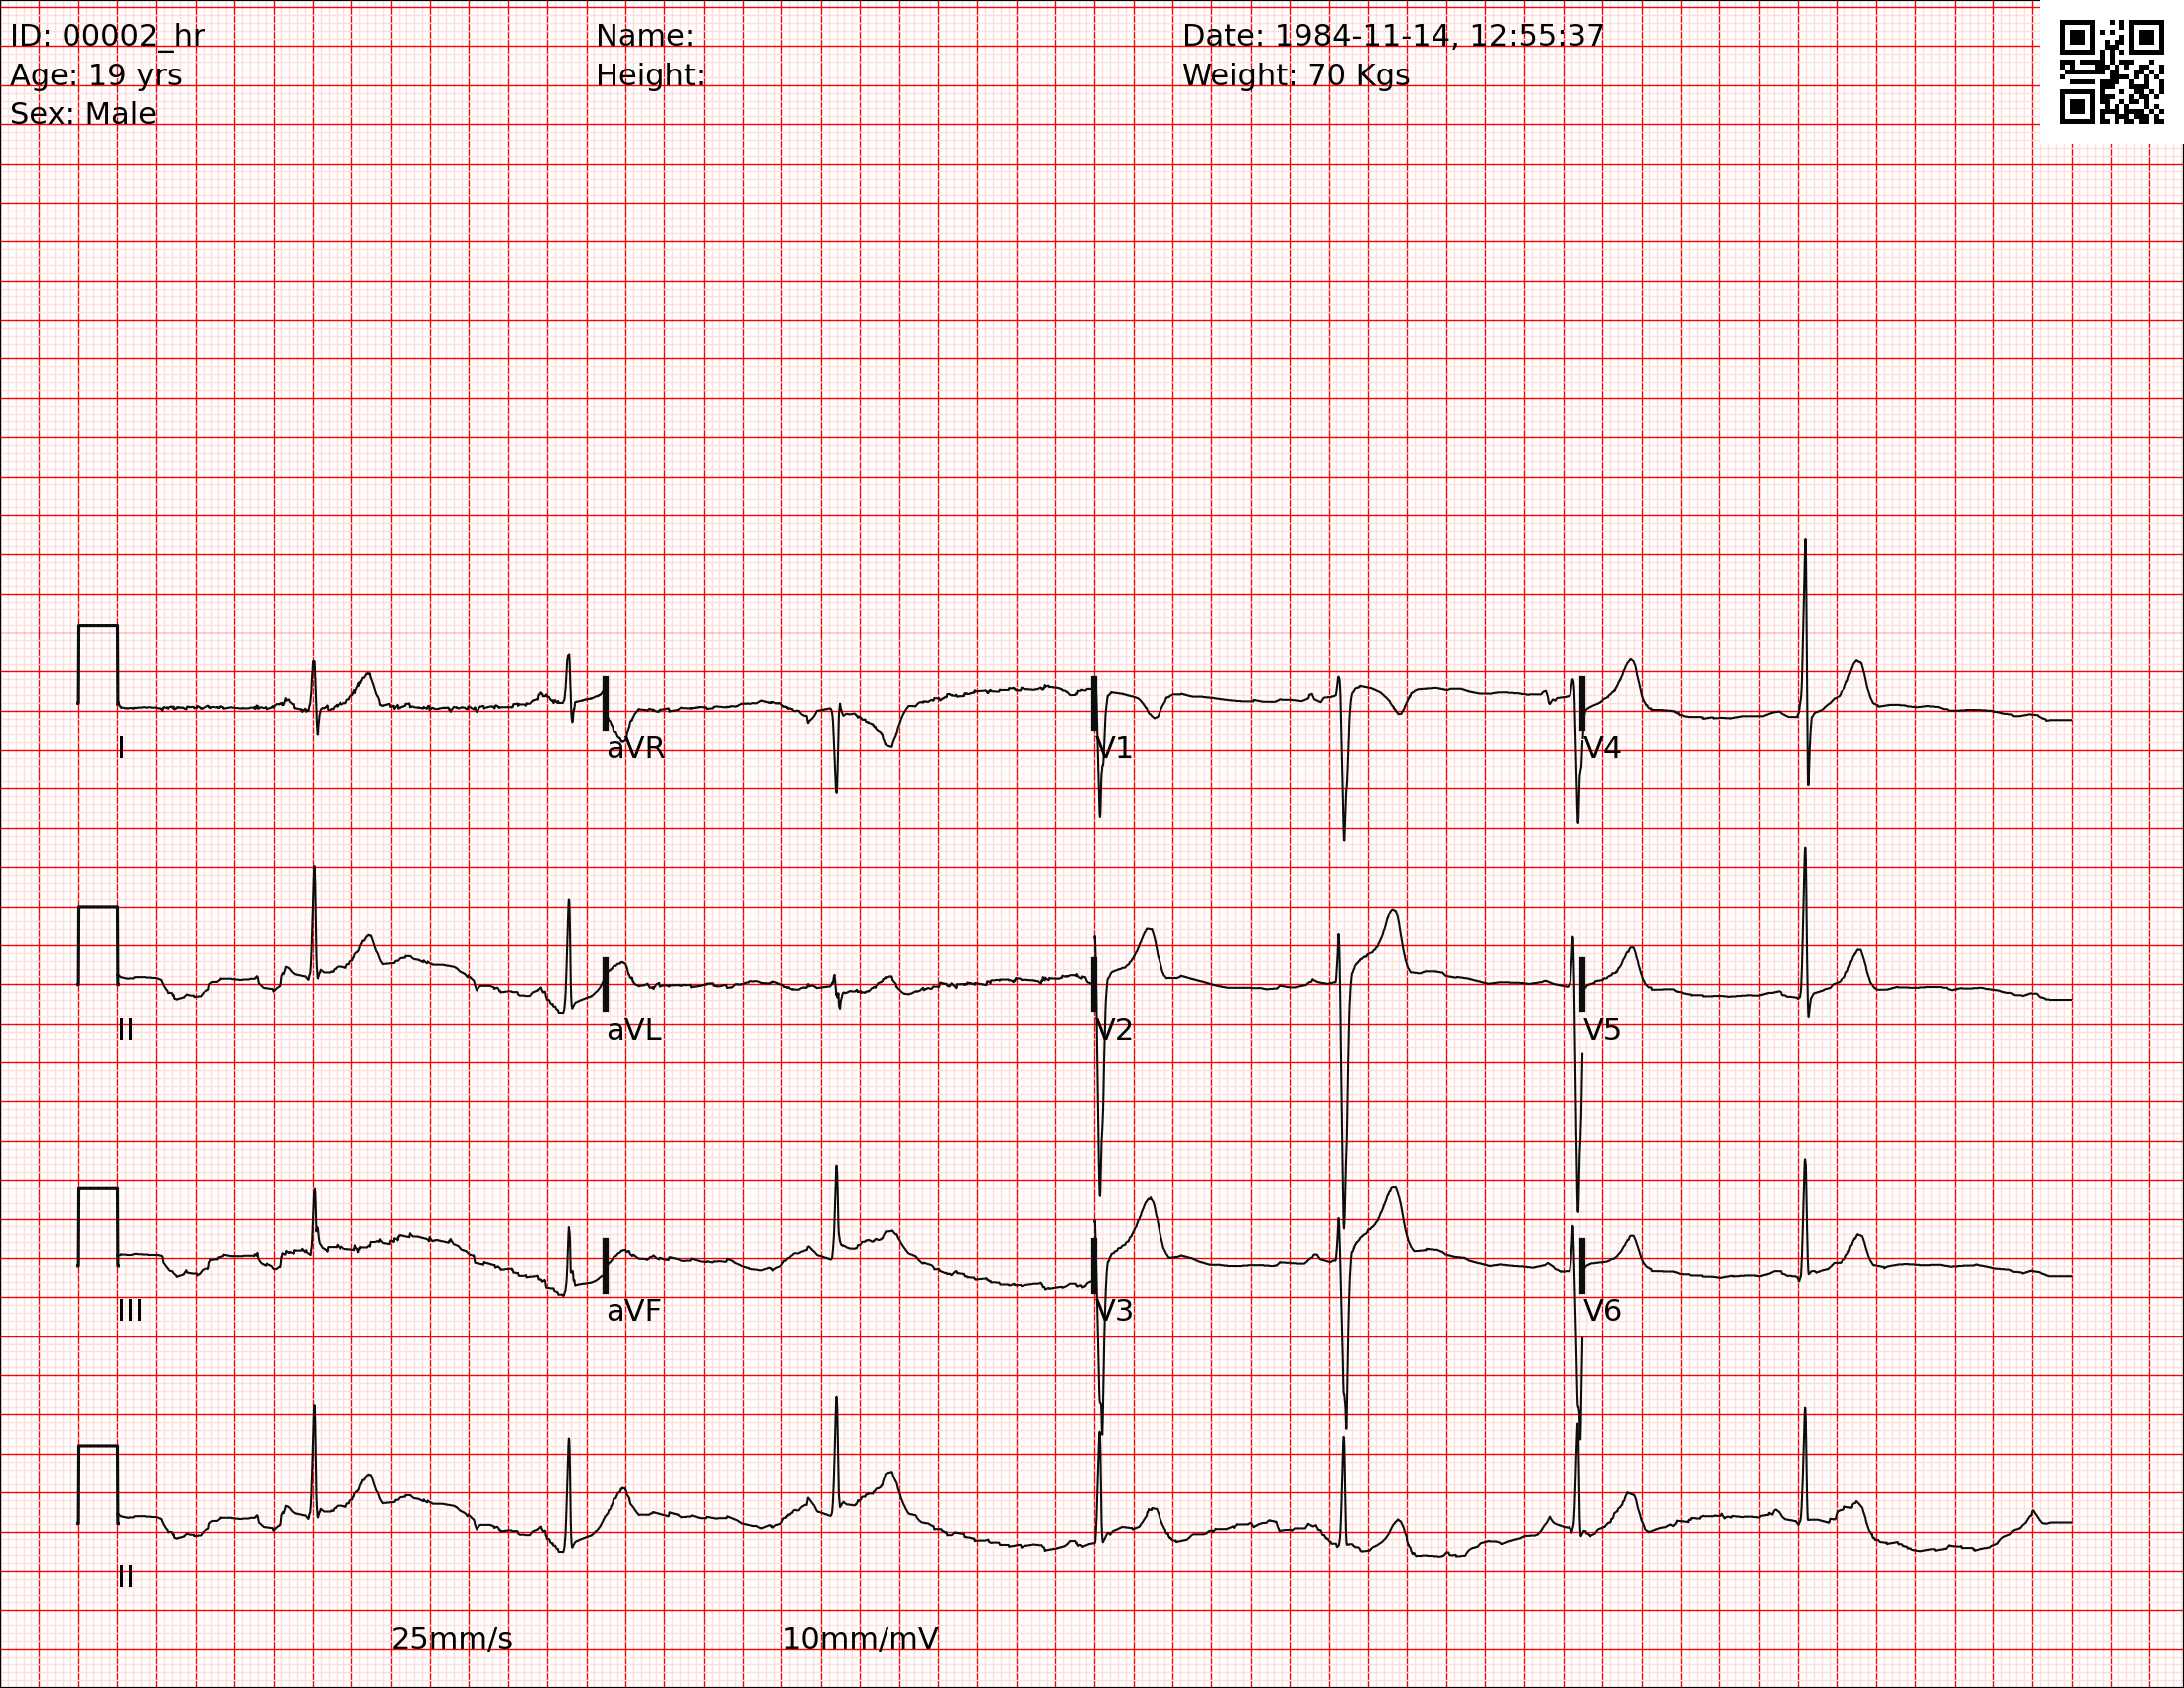
\includegraphics[width=\textwidth]{images/sample_baseline.png}
        \caption{Immagine baseline: nessun artefatto, griglia rossa standard.}
        \label{fig:sample_baseline}
    \end{subfigure}
    \hfill
    \begin{subfigure}[t]{0.48\textwidth}
        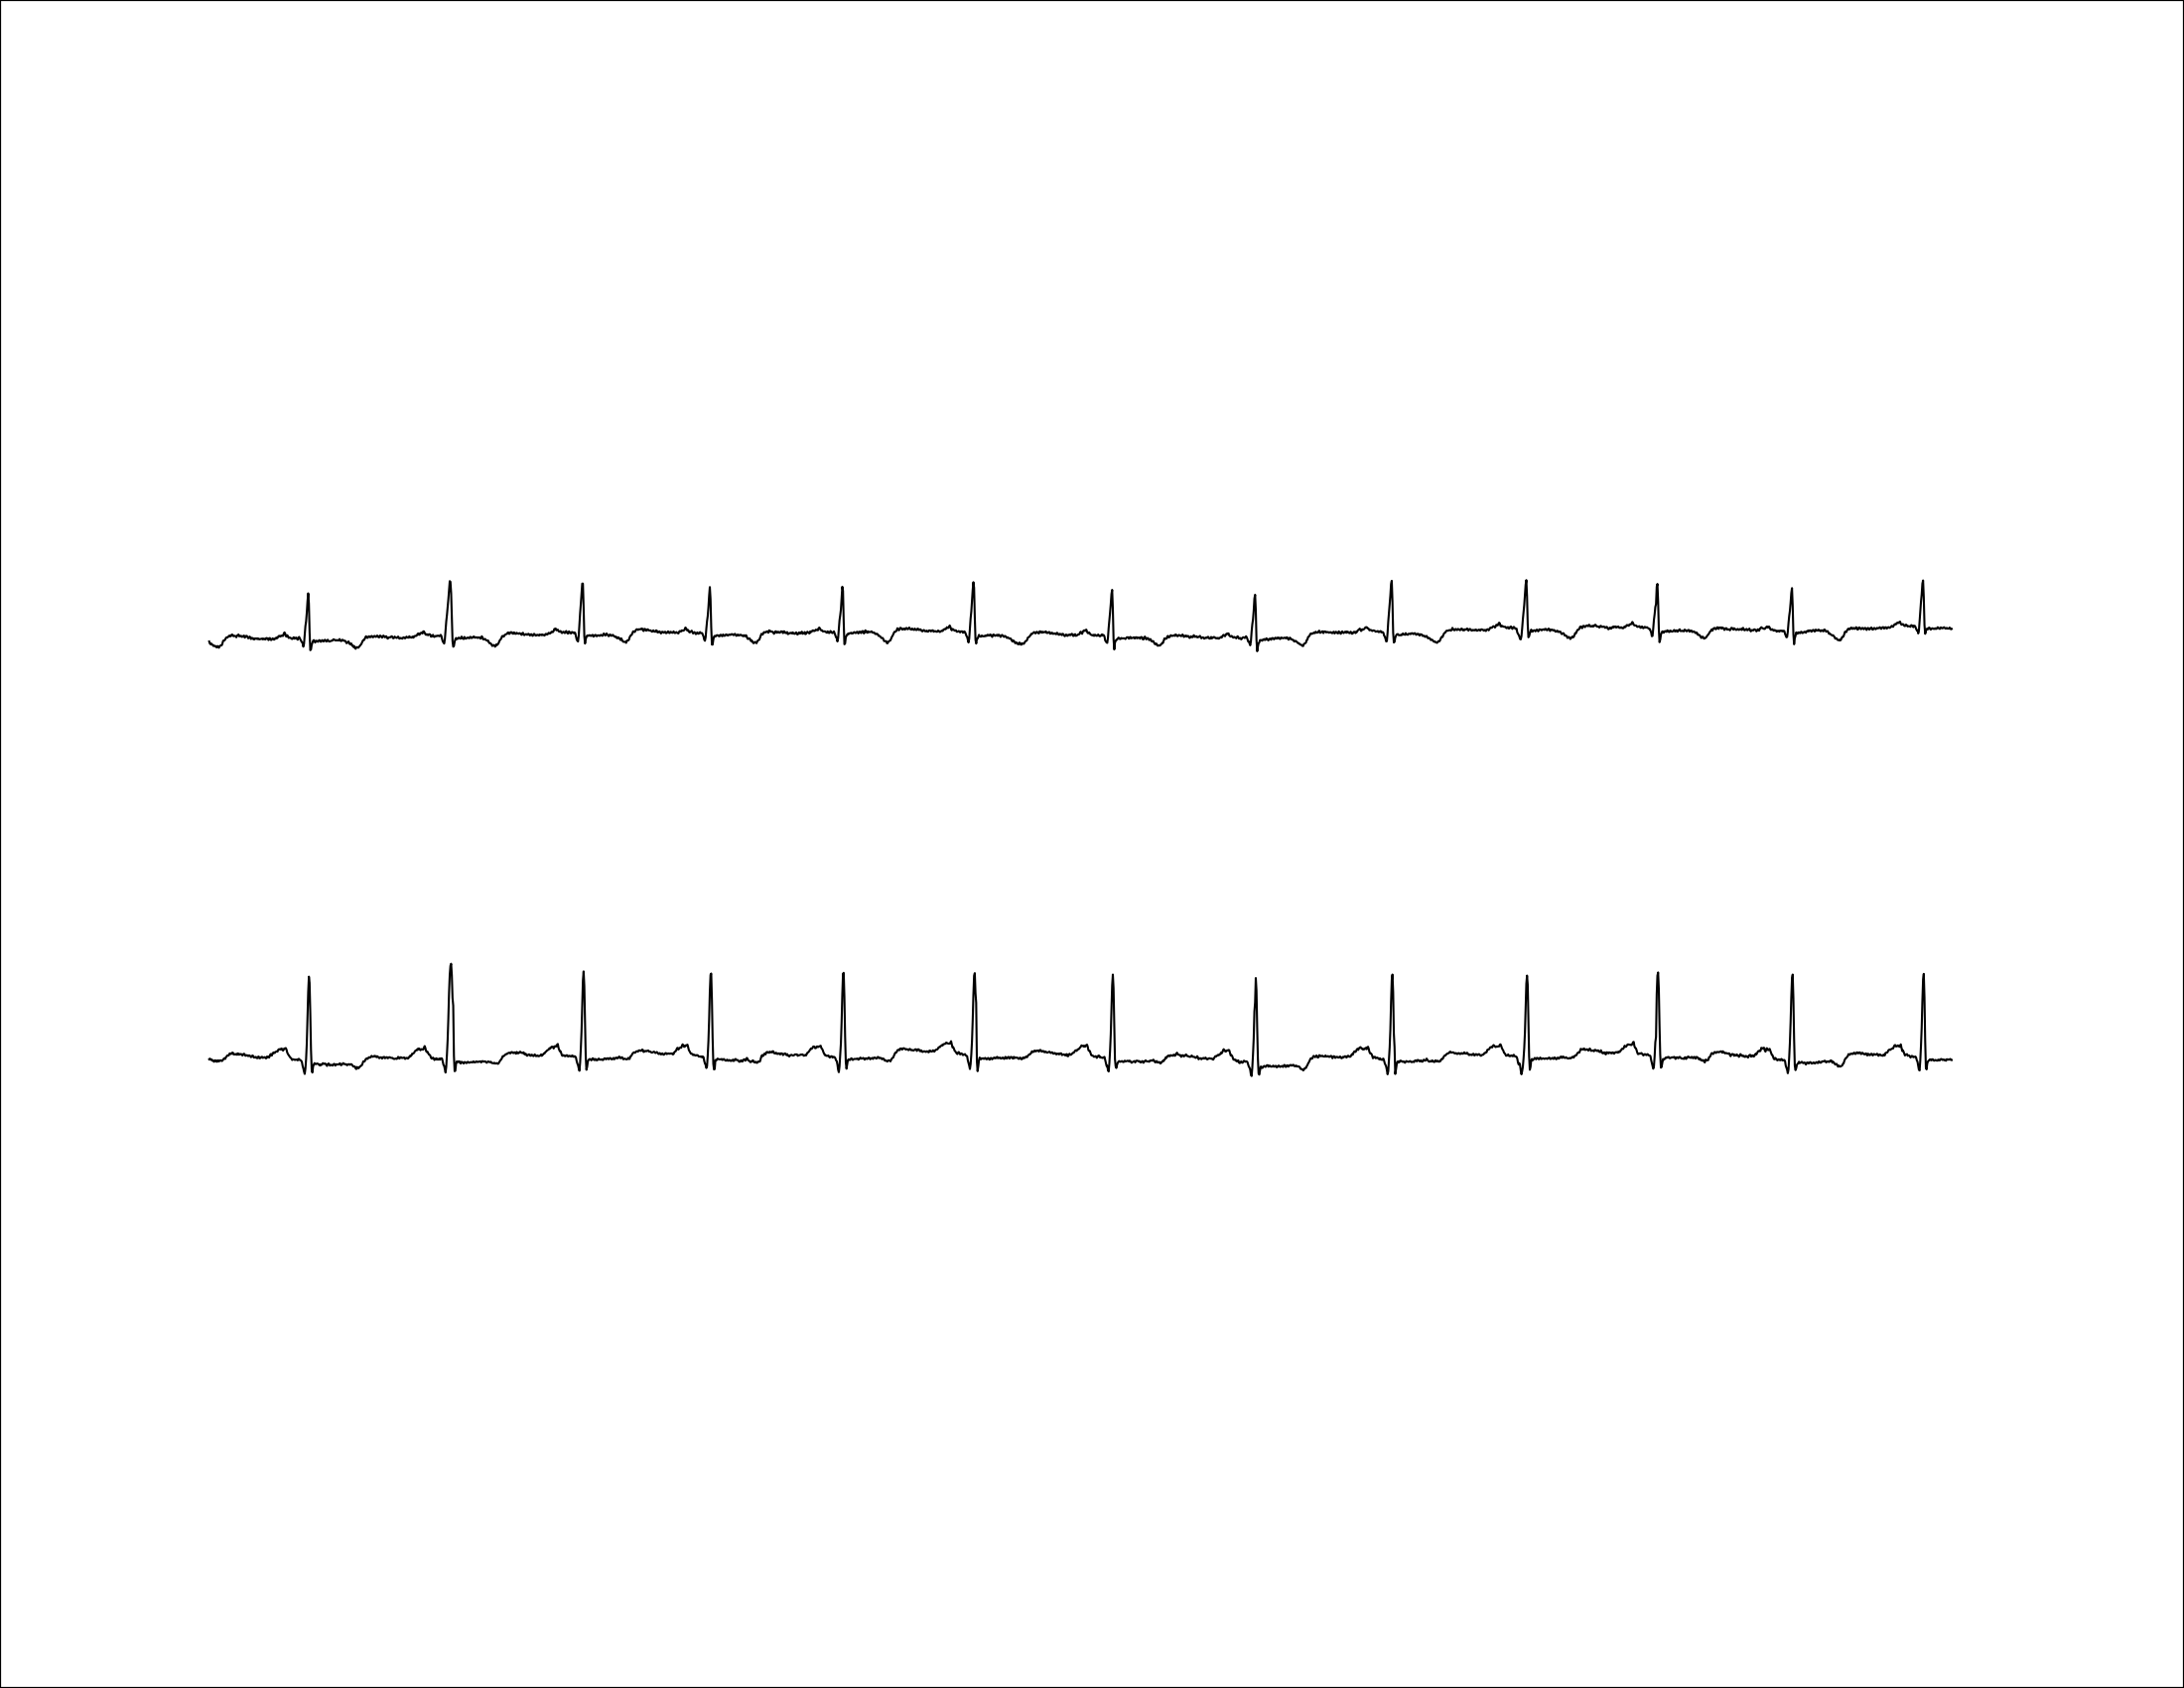
\includegraphics[width=\textwidth]{images/sample_clean.png}
        \caption{Ground truth visiva (\texttt{--generate\_clean}): solo tracciati in nero su sfondo bianco.}
        \label{fig:sample_clean}
    \end{subfigure}
    \caption{Confronto tra immagine sintetica e corrispondente ground truth.}
    \label{fig:sample_pair}
\end{figure}

\begin{figure}[H]
    \centering
    \begin{subfigure}[t]{0.48\textwidth}
        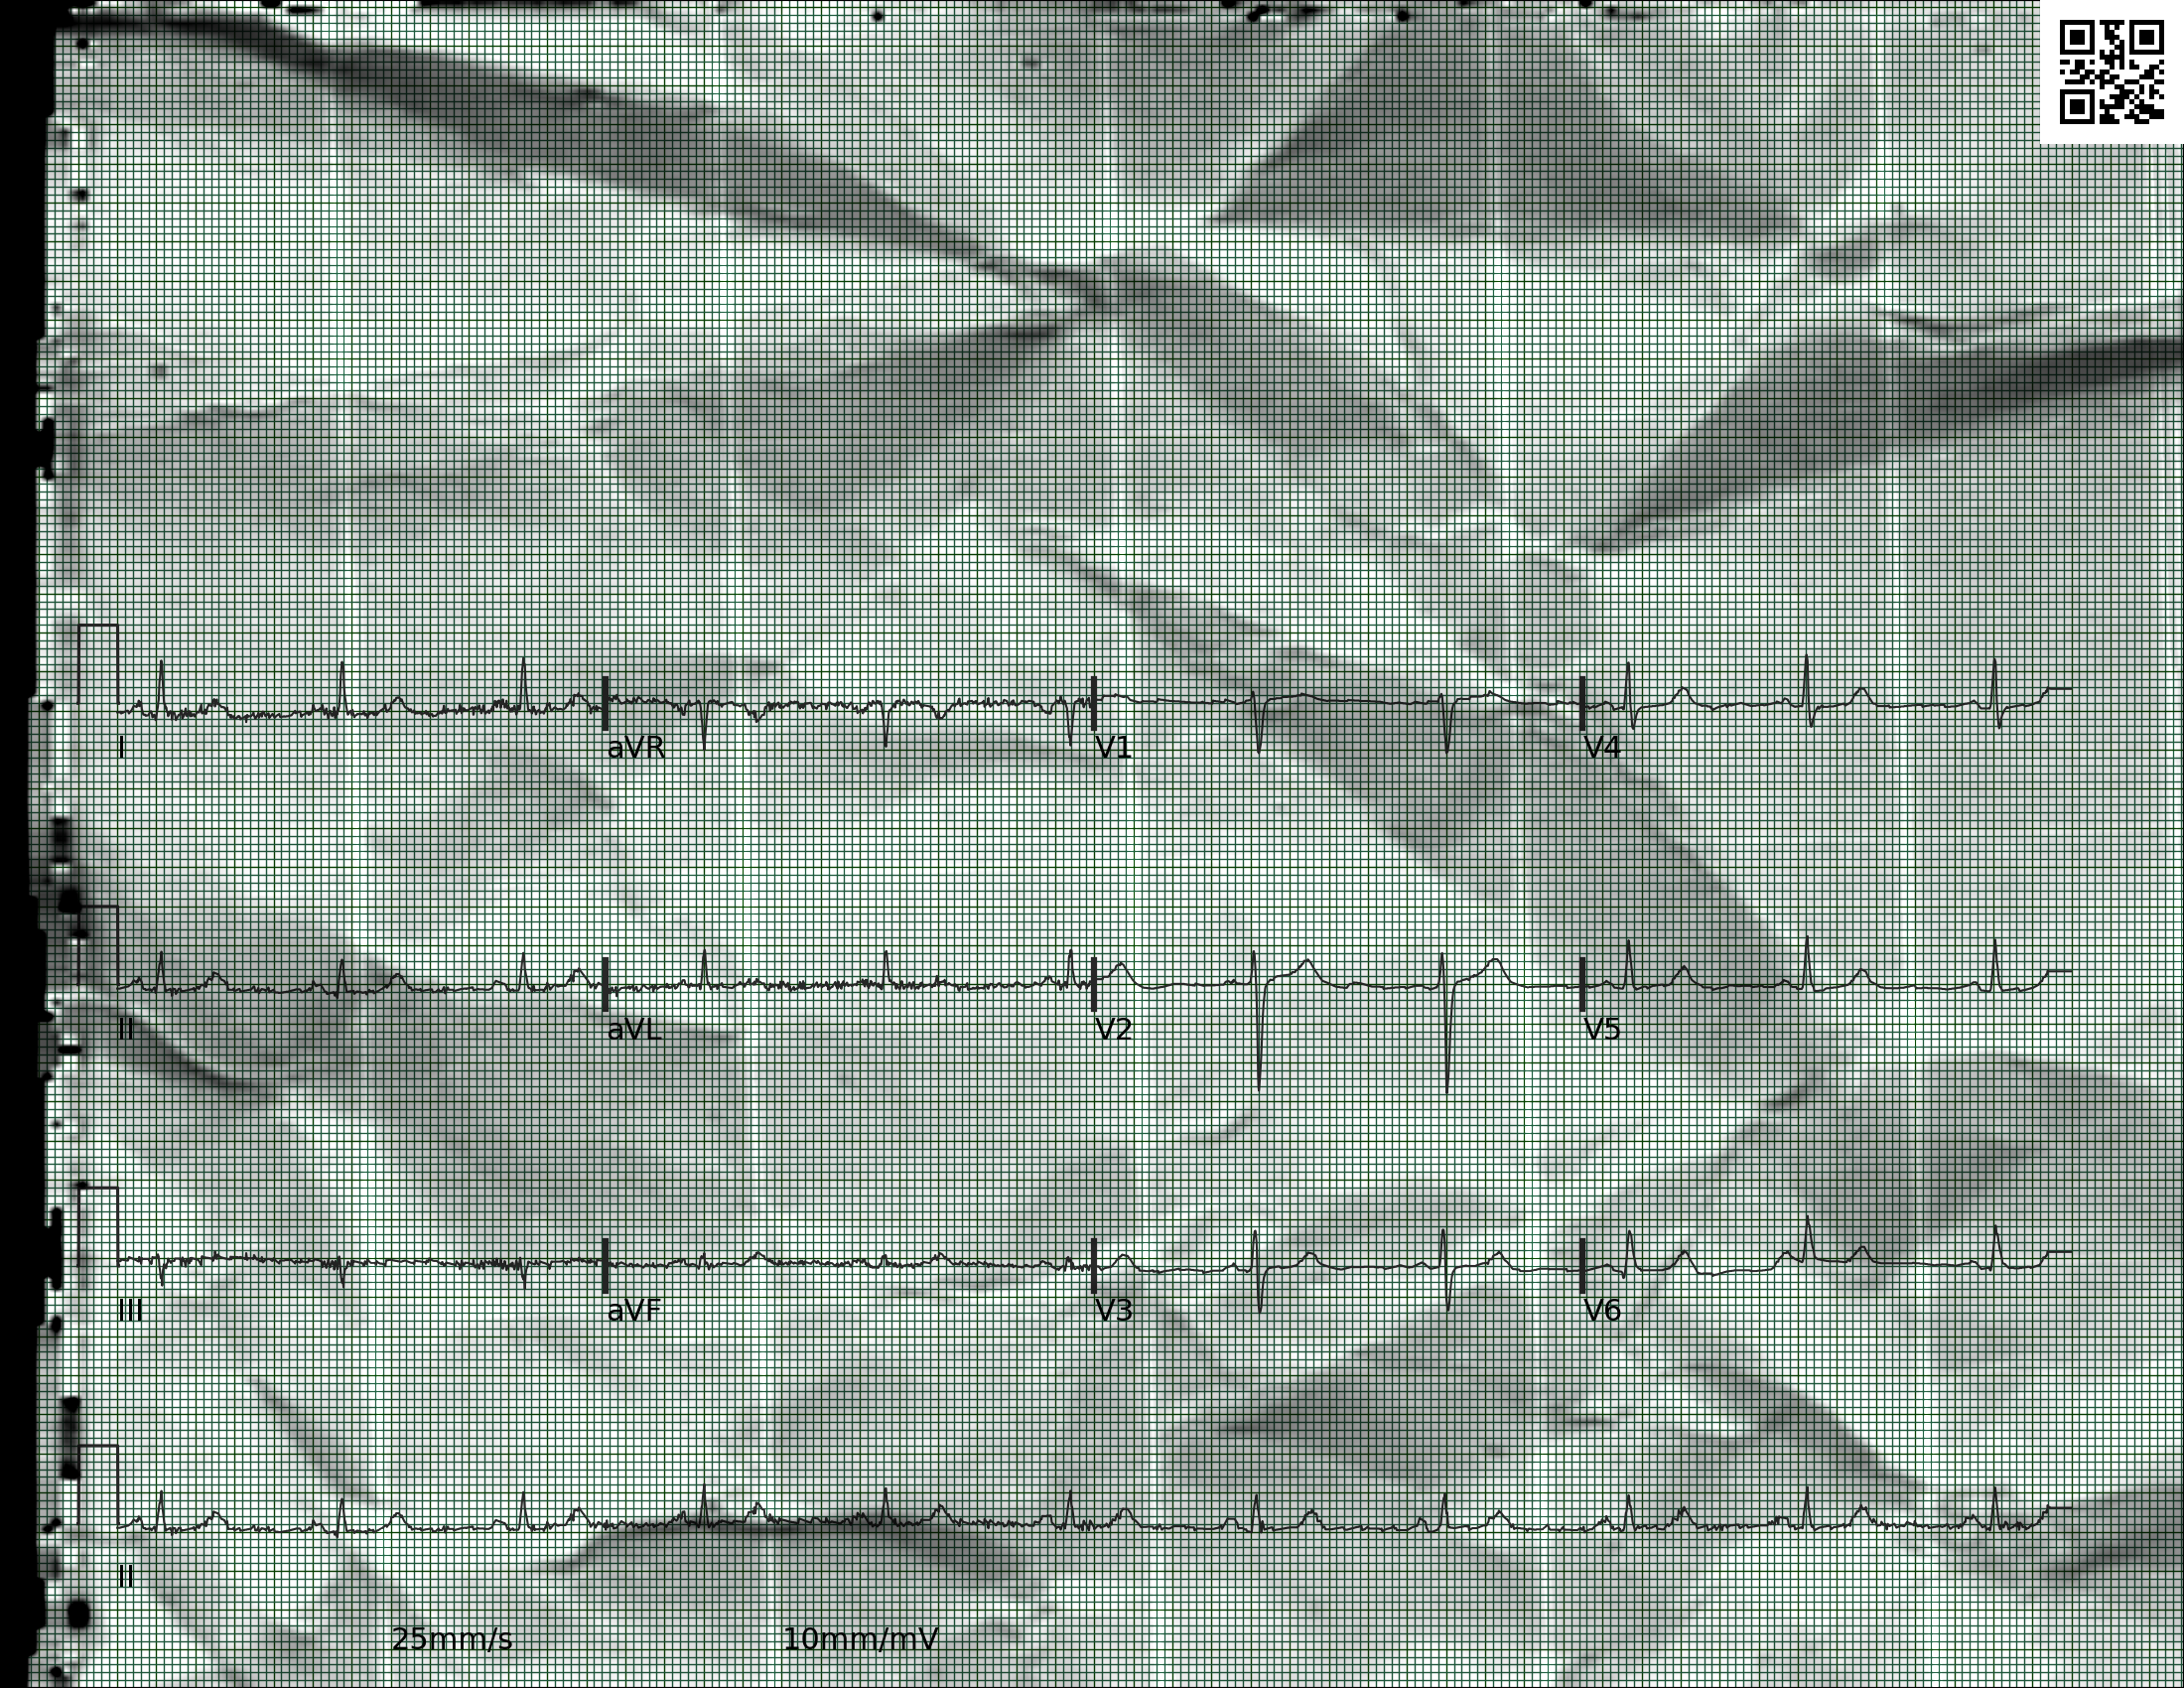
\includegraphics[width=\textwidth]{images/sample_wrinkles.png}
        \caption{Pieghe e rugosità della carta.
        \\}
        \label{fig:sample_wrinkles}
    \end{subfigure}
    \hfill
    \begin{subfigure}[t]{0.48\textwidth}
        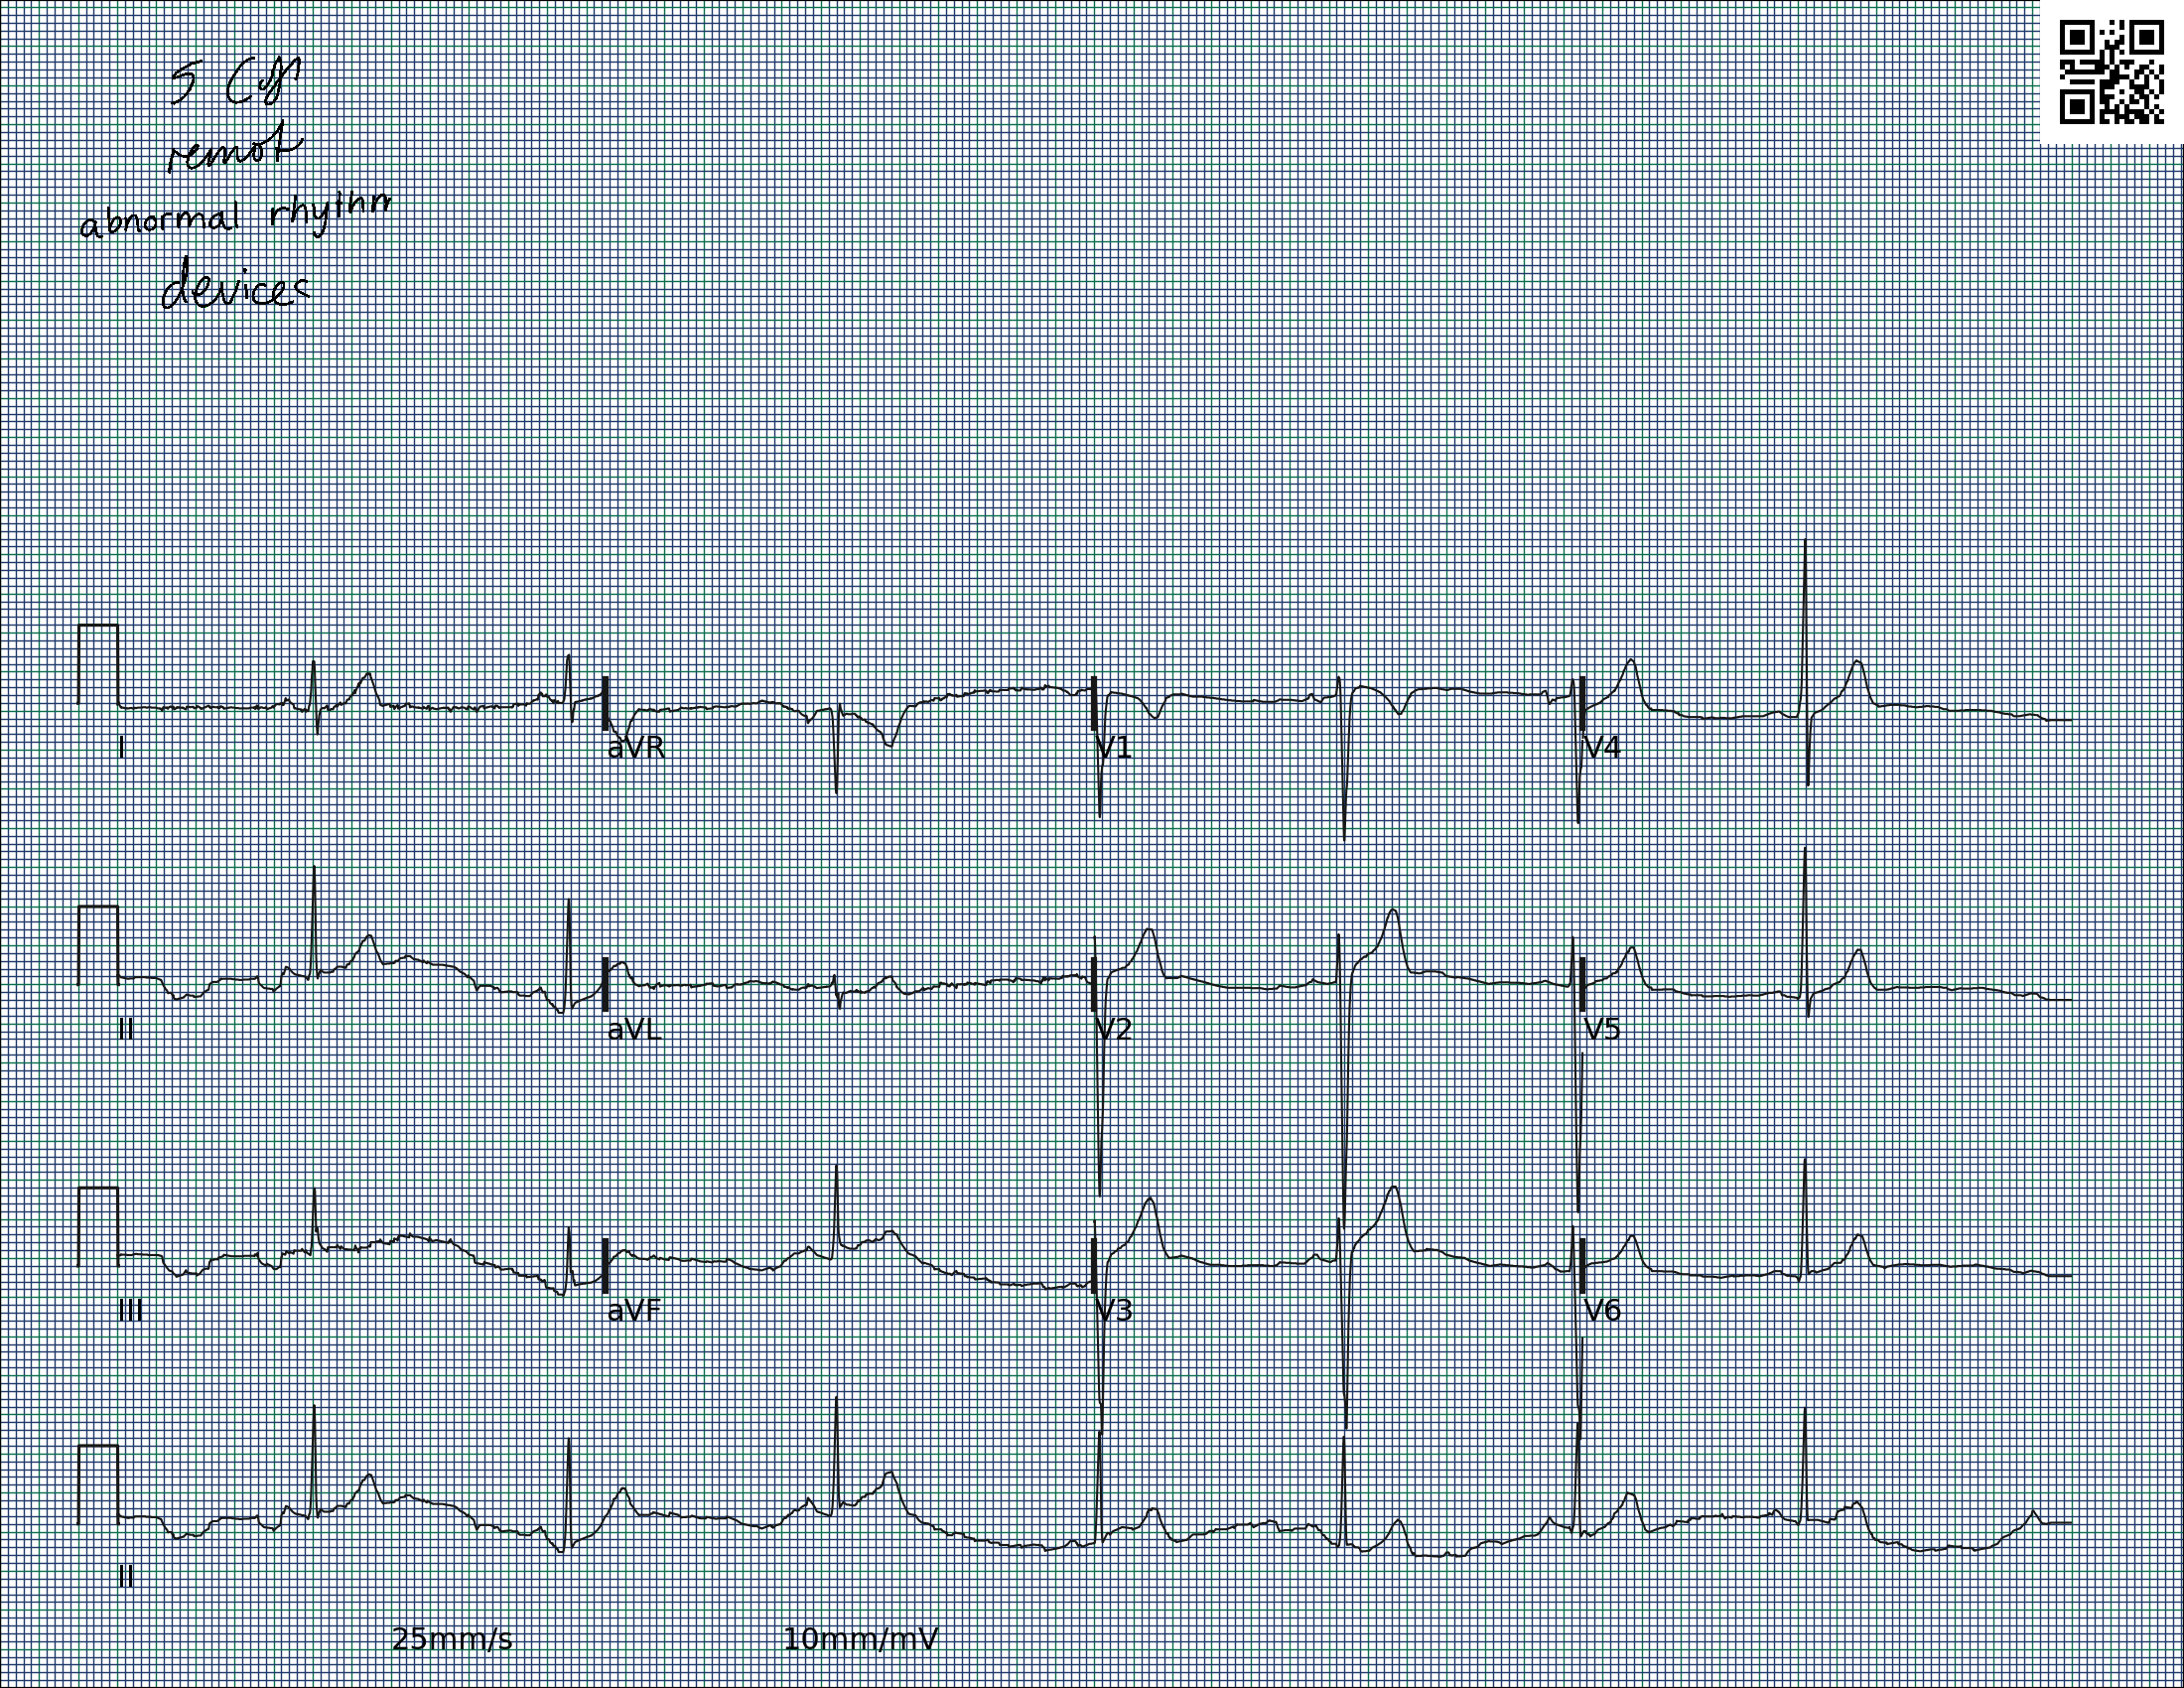
\includegraphics[width=\textwidth]{images/sample_hwtext.png}
        \caption{Testo manoscritto.}
        \label{fig:sample_hwtext}
    \end{subfigure}
    \caption{Esempi di artefatti individuali applicati all'immagine ECG.}
    \label{fig:sample_artifacts}
\end{figure}

\begin{figure}[H]
    \centering
    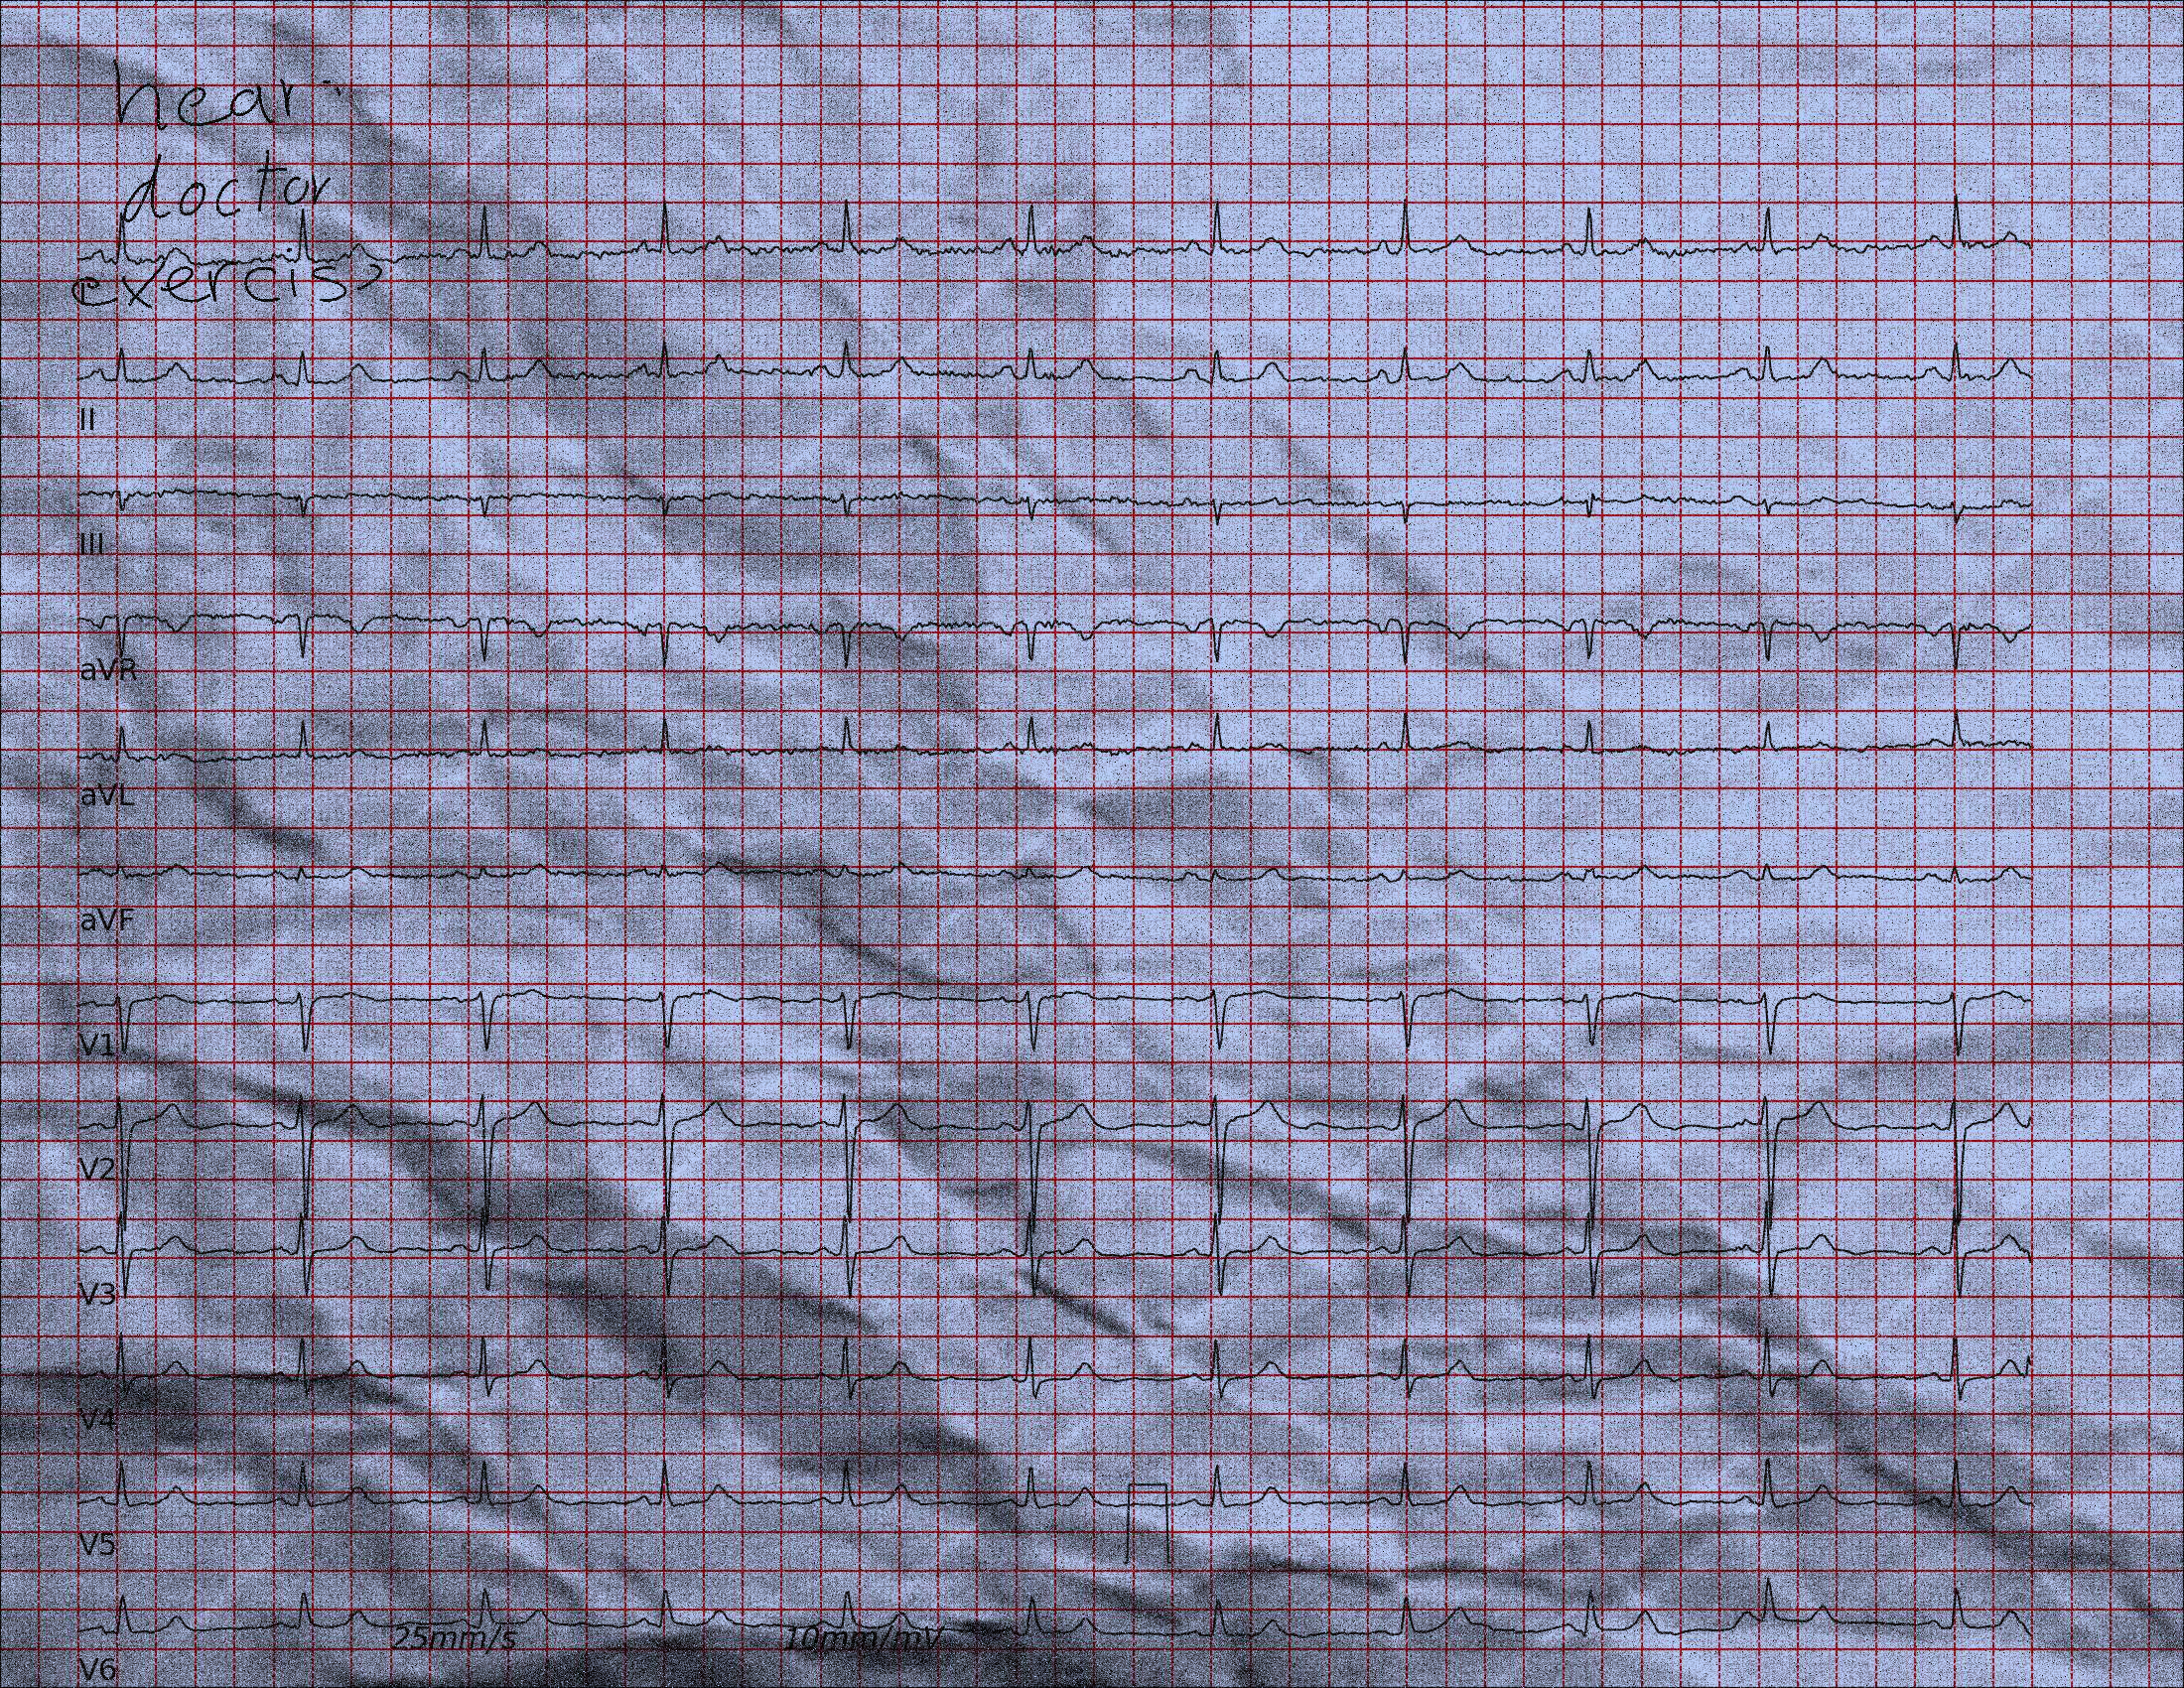
\includegraphics[width=0.7\textwidth]{images/sample_augmented.png}
    \caption{Immagine con artefatti combinati: pieghe della carta e testo manoscritto sovrapposto.}
    \label{fig:sample_augmented}
\end{figure}

\begin{figure}[H]
    \centering
    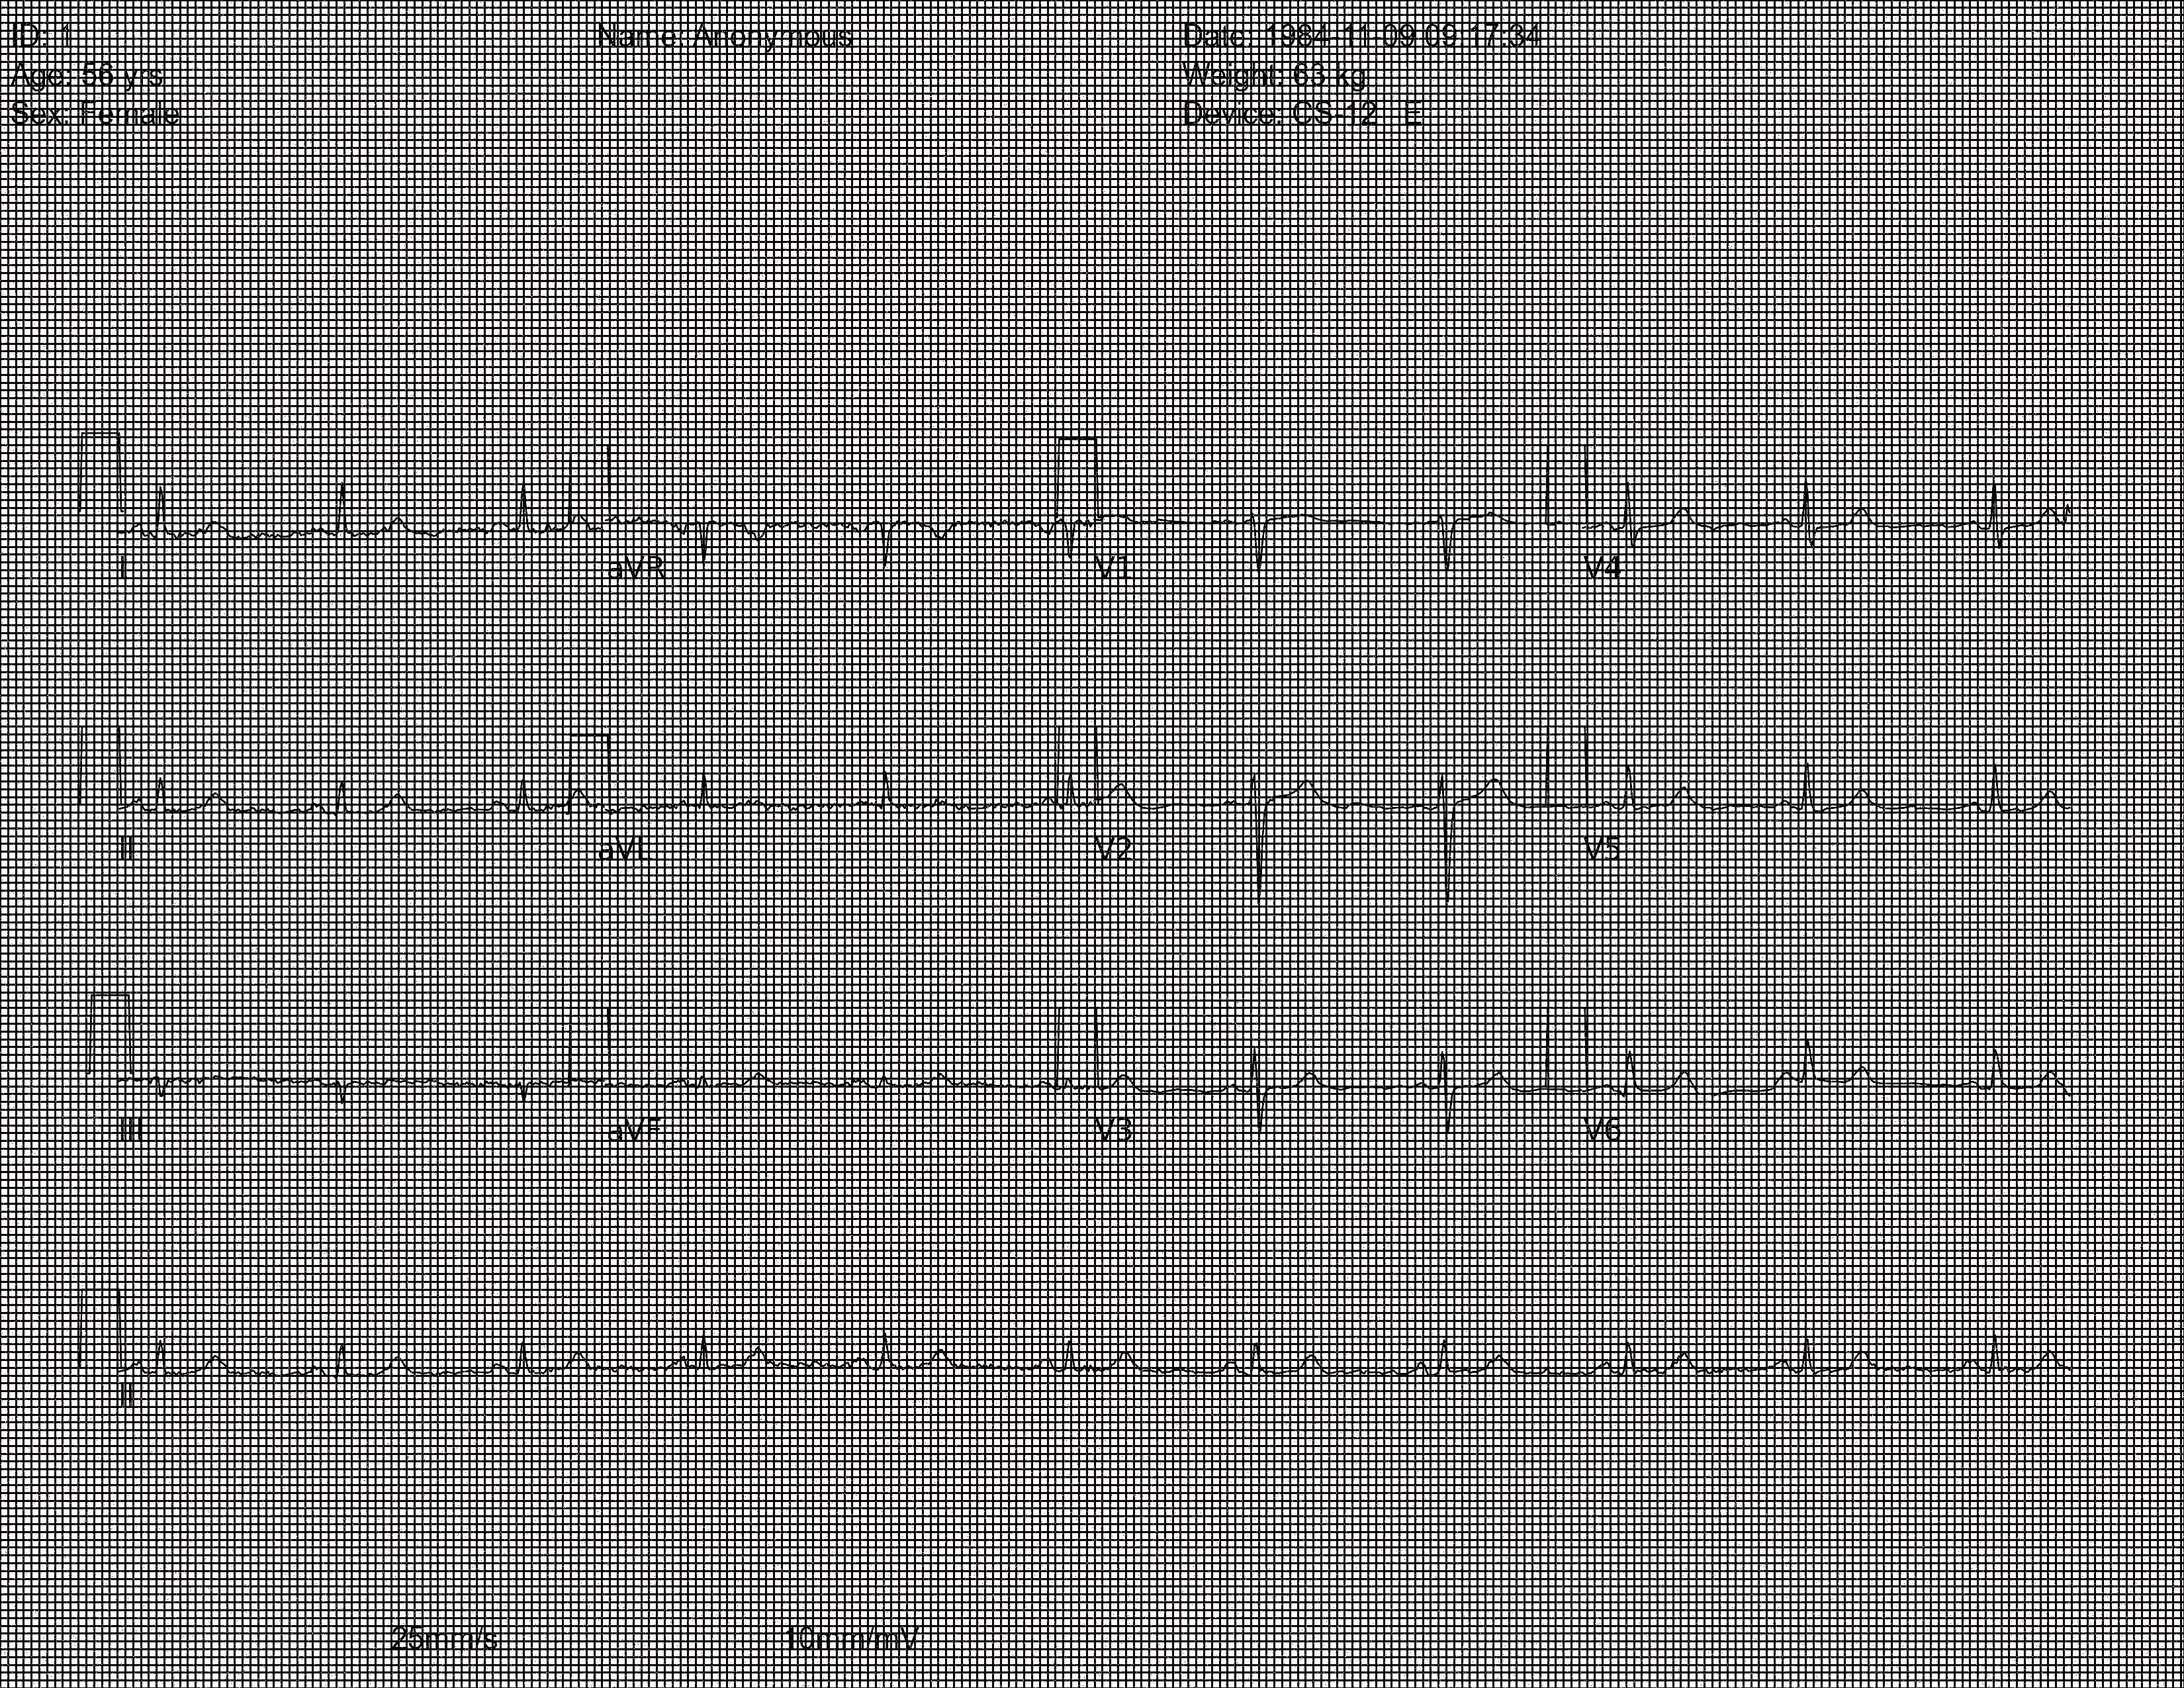
\includegraphics[width=0.7\textwidth]{images/sample_bw.png}
    \caption{Esempio di immagine in bianco e nero (\texttt{--random\_bw}): il colore della griglia viene sostituito con una tonalità di grigio casuale, simulando la variabilità delle stampe monocromatiche.}
    \label{fig:sample_bw}
\end{figure}

\begin{figure}[H]
    \centering
    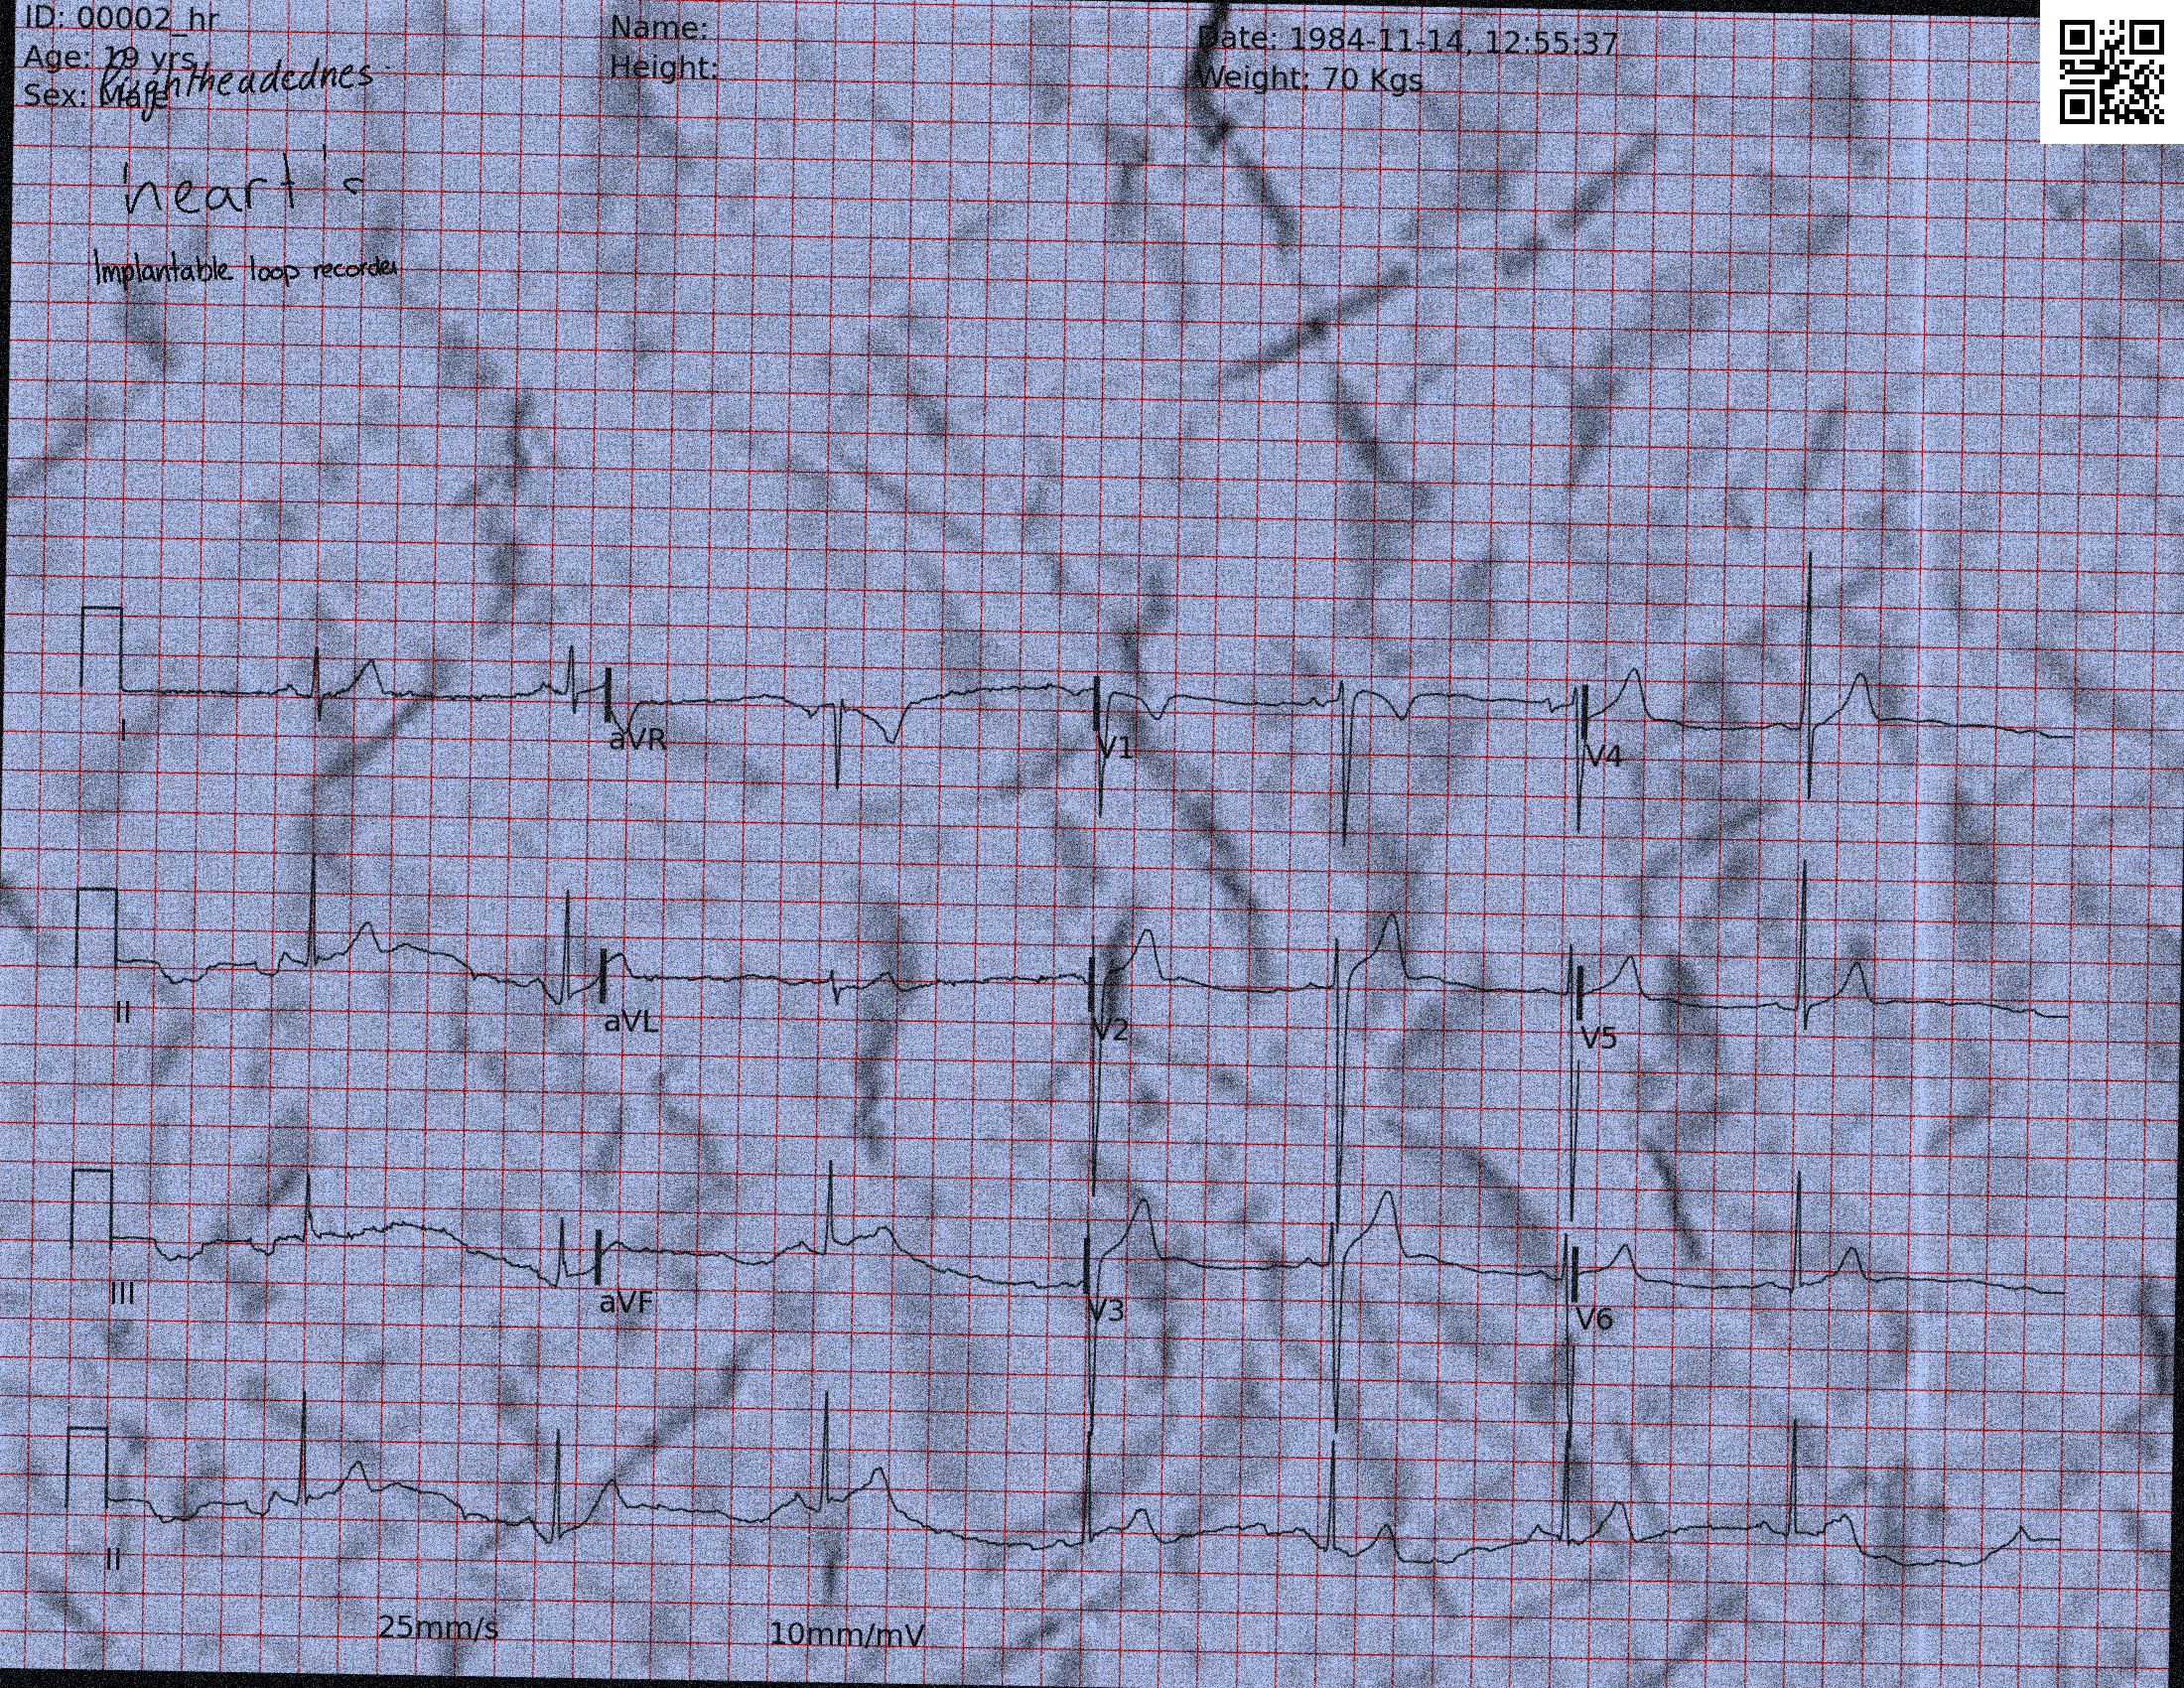
\includegraphics[width=0.7\textwidth]{images/sample_all_artifacts.png}
    \caption{Esempio di output della configurazione completa: griglia colorata casuale, rotazione, rumore, compressione JPEG, pieghe della carta e shift geometrico delle derivazioni.}
    \label{fig:sample_all}
\end{figure}


\section{Benchmark dei Tempi di Generazione}\label{sec:benchmark}

Per la misurazione dei tempi è stato sviluppato lo script \texttt{benchmark.py}, che automatizza l'esecuzione della pipeline nelle diverse configurazioni e raccoglie le statistiche di interesse. Lo script articola la misurazione in due test distinti:

\begin{enumerate}
    \item \textbf{Confronto per configurazione:} esegue in modalità single-process un campione fisso di record per ciascuna delle configurazioni di artefatti (baseline, augmentation, pieghe, testo manoscritto, tutti gli artefatti), misurando il tempo medio per immagine. Un warm-up preventivo sul primo record esclude dalla misurazione il costo di inizializzazione dei modelli TensorFlow.
    \item \textbf{Test di scalabilità:} esegue la configurazione baseline al variare del numero di worker del \texttt{ProcessPoolExecutor} (1, 2, 4, 8, \ldots fino al numero di core disponibili), calcolando speedup ed efficienza parallela rispetto al caso seriale.
\end{enumerate}

I tempi riportati nelle tabelle seguenti sono stati ottenuti su un campione di 20 record (test per configurazione) e 32 record (test di scalabilità) estratti dal dataset PTB-XL con seed fisso (42) per garantire la riproducibilità.

\subsection{Confronto per Configurazione di Artefatti}

La Tabella~\ref{tab:bench_config} riporta il tempo medio di generazione per immagine nelle diverse configurazioni, eseguito in modalità single-process per consentire il confronto diretto con i benchmark della repository originale~\cite{ecgimagekitpaper}.

\begin{table}[H]
\centering
\caption{Tempo medio di generazione per immagine (1 processo, 20 campioni).}
\label{tab:bench_config}
\begin{tabular}{lrr}
\hline
\textbf{Configurazione} & \textbf{Tempo totale (s)} & \textbf{Media/immagine (s)} \\
\hline
Baseline (nessun artefatto)   & 20.20 & 1.010 \\
Augmentation estesa           & 37.14 & 1.857 \\
Pieghe e rugosità             & 37.28 & 1.864 \\
Testo manoscritto             & 74.36 & 3.718 \\
Tutti gli artefatti           & 99.05 & 4.952 \\
\hline
\end{tabular}
\end{table}

\subsection{Scalabilità della Parallelizzazione}

La Tabella~\ref{tab:bench_scale} riporta i tempi di generazione della configurazione baseline al variare del numero di processi paralleli, evidenziando lo speedup ottenuto grazie alla parallelizzazione introdotta in questo lavoro. Il caso a 1 processo corrisponde all'esecuzione seriale della repository originale.

\begin{table}[H]
\centering
\caption{Scalabilità al variare del numero di processi (configurazione baseline, 32 immagini).}
\label{tab:bench_scale}
\begin{tabular}{rrrr}
\hline
\textbf{Processi} & \textbf{Tempo totale (s)} & \textbf{Speedup} & \textbf{Efficienza (\%)} \\
\hline
 1 & 39.06 & $1.00\times$ & 100.0 \\
 2 & 22.10 & $1.77\times$ &  88.4 \\
 4 & 14.27 & $2.74\times$ &  68.4 \\
 8 & 12.87 & $3.03\times$ &  37.9 \\
16 & 15.81 & $2.47\times$ &  15.4 \\
\hline
\end{tabular}
\end{table}

La Figura~\ref{fig:bench_scale} mostra l'andamento di speedup ed efficienza al variare del numero di processi. Lo speedup cresce fino a 8 worker ($3.03\times$) e poi decresce a 16, con un'efficienza che cala progressivamente. Questo comportamento è spiegabile attraverso tre fattori concorrenti.

\paragraph{Hyperthreading e saturazione dei core fisici.}
Il Ryzen 5700X è una CPU con 8 core fisici e 16 thread logici (\textit{Simultaneous Multi-Threading}, SMT). L'hyperthreading permette a ogni core di eseguire due thread in modo interleaved, condividendo le unità di esecuzione: funziona bene quando i thread sono in attesa (I/O, cache miss), ma non quando entrambi richiedono continuamente le stesse risorse aritmetiche. La generazione di immagini ECG è prevalentemente CPU-bound — operazioni su array NumPy, compositing, trasformate — per cui ogni thread occupa il core quasi al 100\%. Passando da 8 a 16 worker si aggiungono solo thread logici sugli stessi core fisici, aumentando la contesa sulle unità di esecuzione anziché aggiungere capacità computazionale reale. Questo spiega il calo effettivo di speedup da $3.03\times$ (8 worker) a $2.47\times$ (16 worker).

\paragraph{Saturazione della banda di memoria.}
Con molti processi attivi simultaneamente, ciascuno carica file WFDB e alloca array NumPy di grandi dimensioni. La memoria DDR4 a canale singolo ha una banda di trasferimento limitata: quando tutti i processi richiedono dati contemporaneamente il bus diventa collo di bottiglia, aumentando le latenze e vanificando parte del parallelismo.

\paragraph{Overhead di coordinazione.}
Il \texttt{ProcessPoolExecutor} serializza gli argomenti di ogni task attraverso \textit{pickling} Python prima di inviarli al worker process, e riceve indietro eventuali eccezioni con lo stesso meccanismo. All'aumentare dei worker cresce anche il numero di processi che il sistema operativo deve schedulare, introducendo context switch e overhead di sincronizzazione che pesano proporzionalmente di più rispetto al lavoro utile svolto.

Il punto di massimo speedup a 8 worker coincide quindi con il numero di core fisici della CPU di test, confermando che la parallelizzazione tramite \texttt{ProcessPoolExecutor} scala in modo efficiente fino al limite hardware reale. Per questo motivo, il sistema è stato configurato per limitare automaticamente il numero di worker ai core fisici tramite \texttt{psutil.cpu\_count(logical=False)}, evitando il degrado prestazionale osservato a 16 worker.

\begin{figure}[H]
\centering
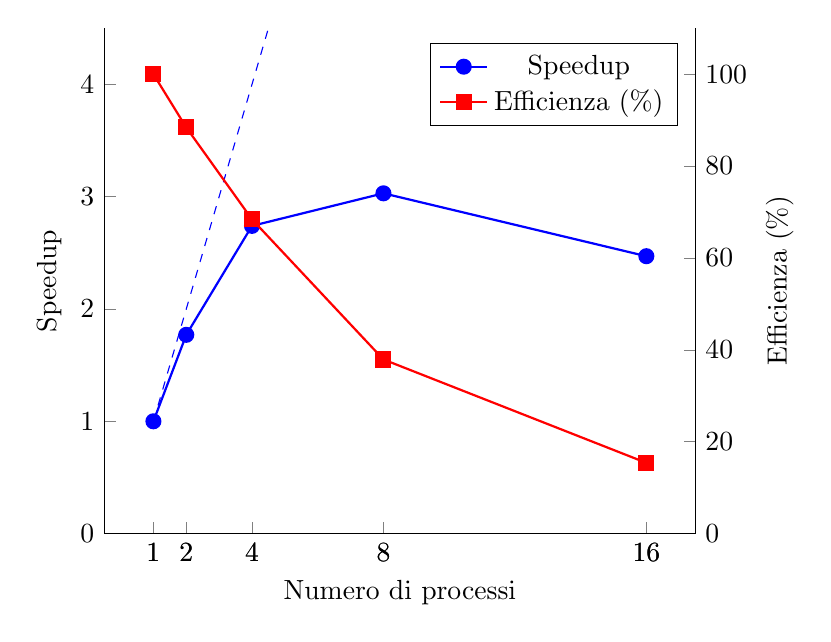
\begin{tikzpicture}
\begin{axis}[
    width=0.75\textwidth,
    height=8cm,
    xlabel={Numero di processi},
    ylabel={Speedup},
    ymin=0, ymax=4.5,
    xtick={1,2,4,8,16},
    ytick={0,1,2,3,4},
    axis y line*=left,
    axis x line*=bottom,
    legend style={at={(0.97,0.97)}, anchor=north east},
    mark size=2.5pt,
]
\addplot[color=blue, mark=*, thick] coordinates {
    (1,  1.00)
    (2,  1.77)
    (4,  2.74)
    (8,  3.03)
    (16, 2.47)
};
\addlegendentry{Speedup}
\addlegendimage{color=red, mark=square*, thick}
\addlegendentry{Efficienza (\%)}

\addplot[color=blue, dashed, thin] coordinates {
    (1, 1) (16, 16)
} node[pos=0.7, above, font=\scriptsize, blue!60] {Speedup ideale};
\end{axis}

\begin{axis}[
    width=0.75\textwidth,
    height=8cm,
    ylabel={Efficienza (\%)},
    ymin=0, ymax=110,
    xtick={1,2,4,8,16},
    axis y line*=right,
    axis x line*=none,
    legend style={draw=none},
    mark size=2.5pt,
]
\addplot[color=red, mark=square*, thick] coordinates {
    (1,  100.0)
    (2,   88.4)
    (4,   68.4)
    (8,   37.9)
    (16,  15.4)
};
\end{axis}
\end{tikzpicture}
\caption{Speedup ed efficienza della parallelizzazione al variare del numero di processi (configurazione baseline, 32 immagini). La linea tratteggiata rappresenta lo speedup ideale (lineare).}
\label{fig:bench_scale}
\end{figure}

\subsection{Confronto con la Repository Originale}

La Tabella~\ref{tab:bench_original} mette a confronto i tempi riportati nella repository originale~\cite{ecgimagekitpaper} (misurati su Apple M2) con quelli ottenuti in questo lavoro sull'hardware di test. I valori non sono direttamente comparabili a causa delle differenze architetturali tra le due piattaforme (Apple M2 con memoria unificata e accelerazione Neural Engine vs AMD Ryzen 5700X, esecuzione CPU-only su Windows); il confronto è riportato a titolo orientativo.

\begin{table}[H]
\centering
\caption{Confronto dei tempi di generazione con la repository originale (Apple M2 vs hardware di test).}
\label{tab:bench_original}
\begin{tabular}{lrr}
\hline
\textbf{Configurazione} & \textbf{Apple M2 (s)} & \textbf{Questo lavoro (s)} \\
\hline
Baseline                          & 0.72 & 1.010 \\
Baseline + intestazione stampata  & 0.87 & 1.112  \\
Testo manoscritto                 & 6.25 & 3.718 \\
Pieghe e rugosità                 & 0.92 & 1.864 \\
Augmentation (rumore e rotazione) & 2.65 & 1.857 \\
Tutti gli artefatti               & 7.75 & 4.952 \\
\hline
\end{tabular}
\end{table}

La Figura~\ref{fig:bench_comparison} visualizza il confronto per le configurazioni disponibili in entrambe le misurazioni. I risultati riflettono le differenze architetturali tra le due piattaforme.

La \textbf{baseline} è più lenta sull'hardware di test: senza artefatti, la generazione si riduce a puro rendering (matplotlib, compositing NumPy), un workload prevalentemente memory-bound che beneficia della memoria unificata dell'Apple M2 (banda $\sim$100~GB/s) e delle sue elevate prestazioni single-core su operazioni vettoriali ARM~NEON.

Le configurazioni con \textbf{augmentation} e \textbf{testo manoscritto} risultano invece più veloci: la libreria \texttt{imgaug} sfrutta le istruzioni AVX2 e FMA dell'architettura x86 del Ryzen~5700X per le operazioni su array, offrendo un vantaggio rispetto all'equivalente ARM; per il testo manoscritto pesa anche la differenza nelle ottimizzazioni del runtime TensorFlow tra le due piattaforme.

La configurazione con sole \textbf{pieghe} è leggermente più lenta: l'algoritmo di image quilting è computazionalmente intenso ma non beneficia di istruzioni SIMD specifiche come l'augmentation, rendendo la banda di memoria il fattore discriminante.

Va sottolineato che il confronto è effettuato in modalità single-process. Grazie alla parallelizzazione introdotta in questo lavoro, attivando 8 worker il throughput effettivo scala di $3.03\times$: la baseline passa da 1.010~s a $\sim$0.33~s per immagine, scendendo abbondantemente al di sotto del valore misurato sull'Apple~M2. Analogamente, la configurazione con tutti gli artefatti passa da 4.952~s a $\sim$1.63~s per immagine, un risultato non raggiungibile dalla repository originale, che non supporta l'elaborazione parallela.

\begin{figure}[H]
\centering
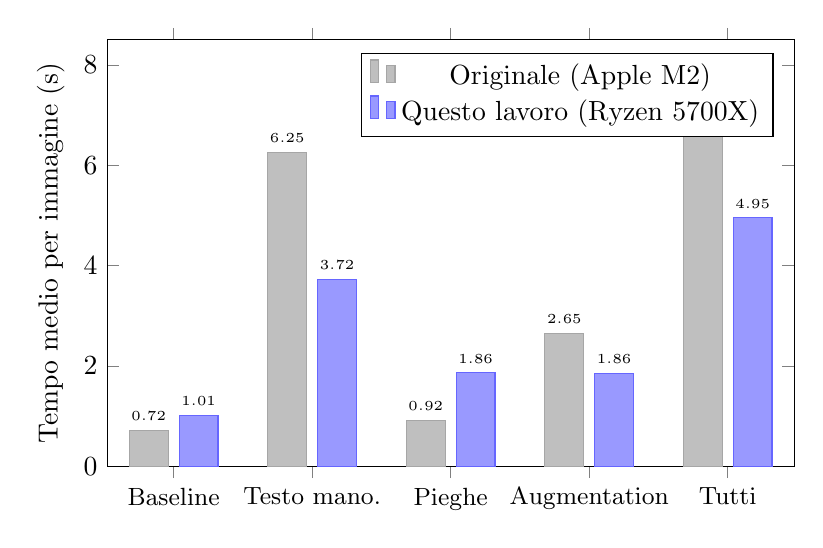
\begin{tikzpicture}
\begin{axis}[
    width=0.85\textwidth,
    height=7cm,
    ybar=4pt,
    bar width=14pt,
    xlabel={},
    ylabel={Tempo medio per immagine (s)},
    ymin=0, ymax=8.5,
    xtick=data,
    xticklabels={Baseline, Testo mano., Pieghe, Augmentation, Tutti},
    xticklabel style={font=\small},
    legend style={at={(0.97,0.97)}, anchor=north east},
    nodes near coords,
    nodes near coords style={font=\tiny, /pgf/number format/fixed, /pgf/number format/precision=2},
    enlarge x limits=0.12,
]
\addplot[fill=gray!50, draw=gray!70] coordinates {
    (1, 0.72)
    (2, 6.25)
    (3, 0.92)
    (4, 2.65)
    (5, 7.75)
};
\addlegendentry{Originale (Apple M2)}

\addplot[fill=blue!40, draw=blue!60] coordinates {
    (1, 1.010)
    (2, 3.718)
    (3, 1.864)
    (4, 1.857)
    (5, 4.952)
};
\addlegendentry{Questo lavoro (Ryzen 5700X)}
\end{axis}
\end{tikzpicture}
\caption{Confronto dei tempi medi per immagine tra la repository originale (Apple M2) e questo lavoro (AMD Ryzen 5700X, CPU-only). La configurazione ``Baseline + intestazione stampata'' è esclusa in quanto non misurata in questo lavoro.}
\label{fig:bench_comparison}
\end{figure}

\section{Struttura dell'Output}

Per ogni record ECG elaborato il sistema produce i seguenti file nella directory di output, replicando la struttura di sottodirectory dell'input. Il nome base di ciascun file rispecchia il record sorgente: \texttt{<id>\_lr} per i record a bassa risoluzione (100~Hz, dataset PTB-XL \texttt{records100}) e \texttt{<id>\_hr} per quelli ad alta risoluzione (500~Hz, \texttt{records500}). Ad esempio, dal record \texttt{00001\_lr} si ottengono i file seguenti:

\begin{itemize}
    \item \textbf{Immagine PNG sintetica} (\texttt{<id>\_lr-<n>.png}): l'immagine principale con griglia, tracciati, etichette e tutti gli artefatti configurati. Il suffisso \texttt{-<n>} (a partire da 0) distingue le varianti generate dallo stesso record.
    \item \textbf{Immagine PNG pulita} (\texttt{<id>\_lr-<n>\_clean.png}, opzionale): la ground truth visiva, generata quando \texttt{--generate\_clean} è attivo. Contiene solo i tracciati in nero su sfondo bianco, senza griglia né artefatti.
    \item \textbf{File WFDB aggiornati} (\texttt{<id>\_lr.hea} e \texttt{<id>\_lr.dat}): copia dei file di segnale originali con la segmentazione temporale applicata e, se \texttt{--mask\_unplotted\_samples} è attivo, i campioni non rappresentati mascherati con \texttt{NaN}.
    \item \textbf{File JSON di configurazione} (\texttt{<id>\_lr-<n>.json}, opzionale): serializza i parametri di generazione e le annotazioni geometriche (bounding box delle derivazioni e dei nomi, coordinate pixel dei segnali plottati) secondo il livello di dettaglio configurato tramite \texttt{--store\_config}.
\end{itemize}

\vspace{4mm}
La coppia immagine sintetica / ground truth visiva, combinata con le annotazioni JSON, rende il dataset direttamente utilizzabile per tre tipologie di task supervisionati: \textbf{segmentazione semantica} (separare segnale da griglia e artefatti), \textbf{object detection} (localizzare le derivazioni tramite bounding box) e \textbf{digitalizzazione} (ricostruire il segnale digitale dall'immagine tramite le coordinate pixel plottate).